% Editable native annotations around unchanged verified IDE photographs.
\par
\begin{figure}[htbp]
  \centering
  \sbox0{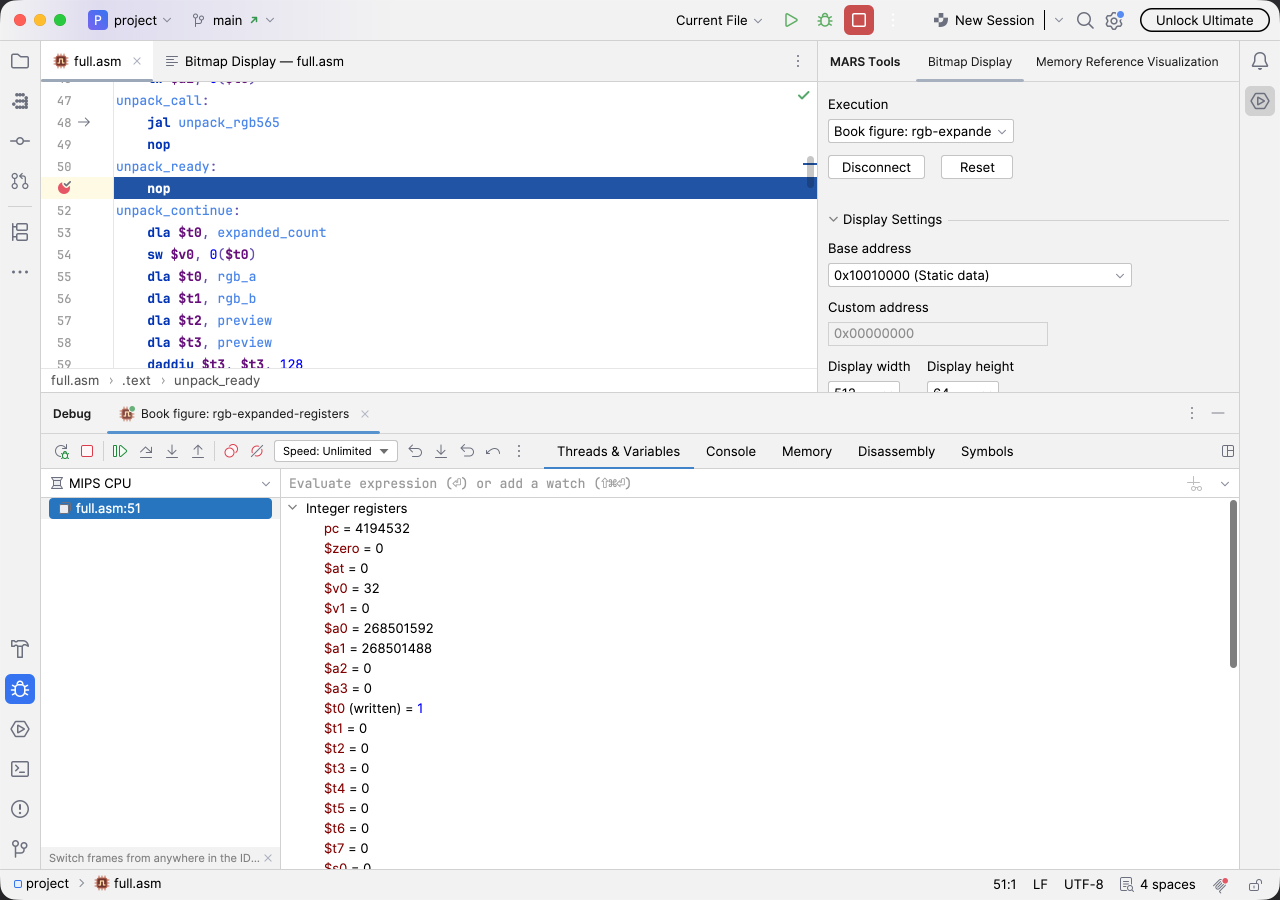
\includegraphics[artifact]{packages/019-rgb-formats/captures/f02/registers.png}}
  \sbox2{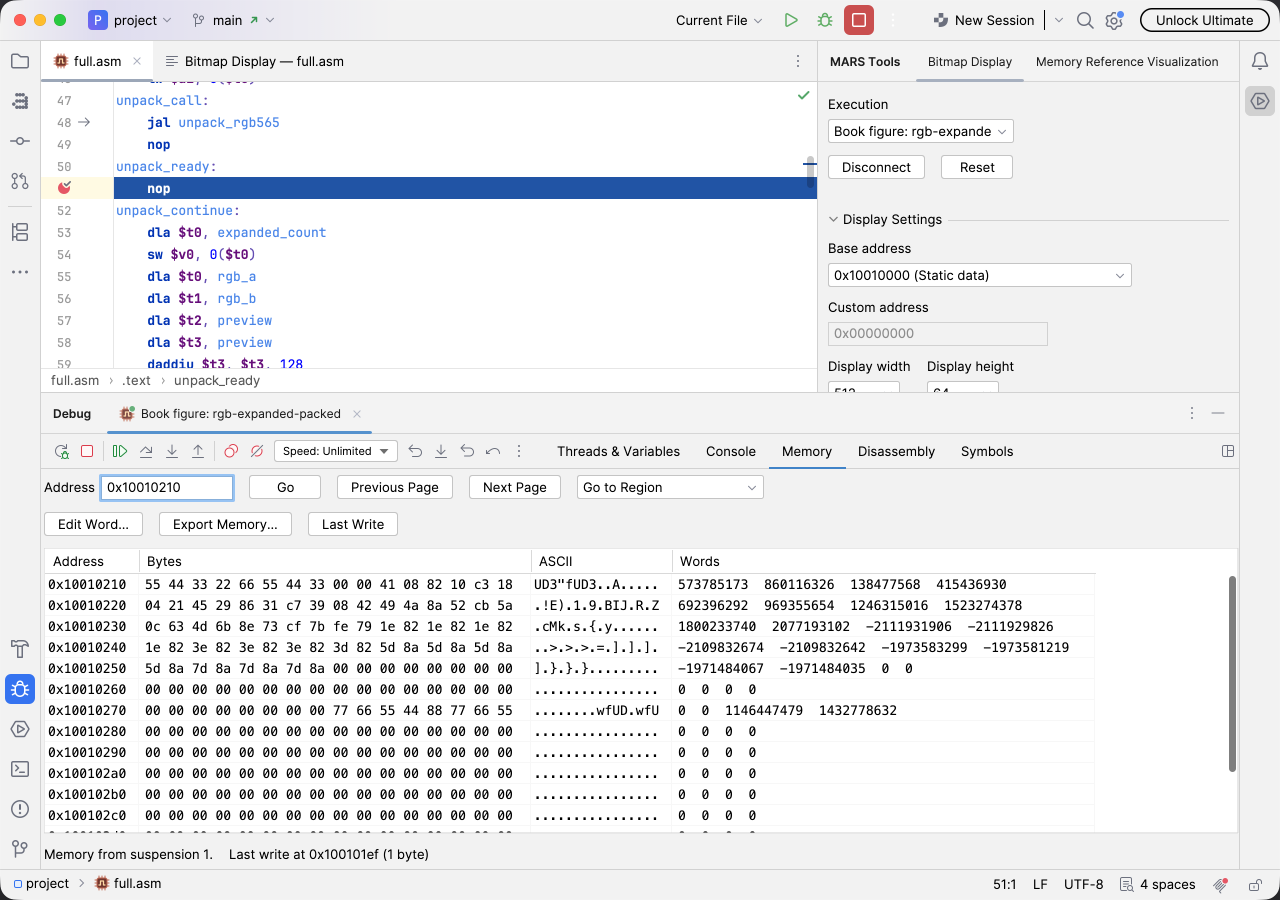
\includegraphics[artifact]{packages/019-rgb-formats/captures/f02/packed.png}}
  \sbox4{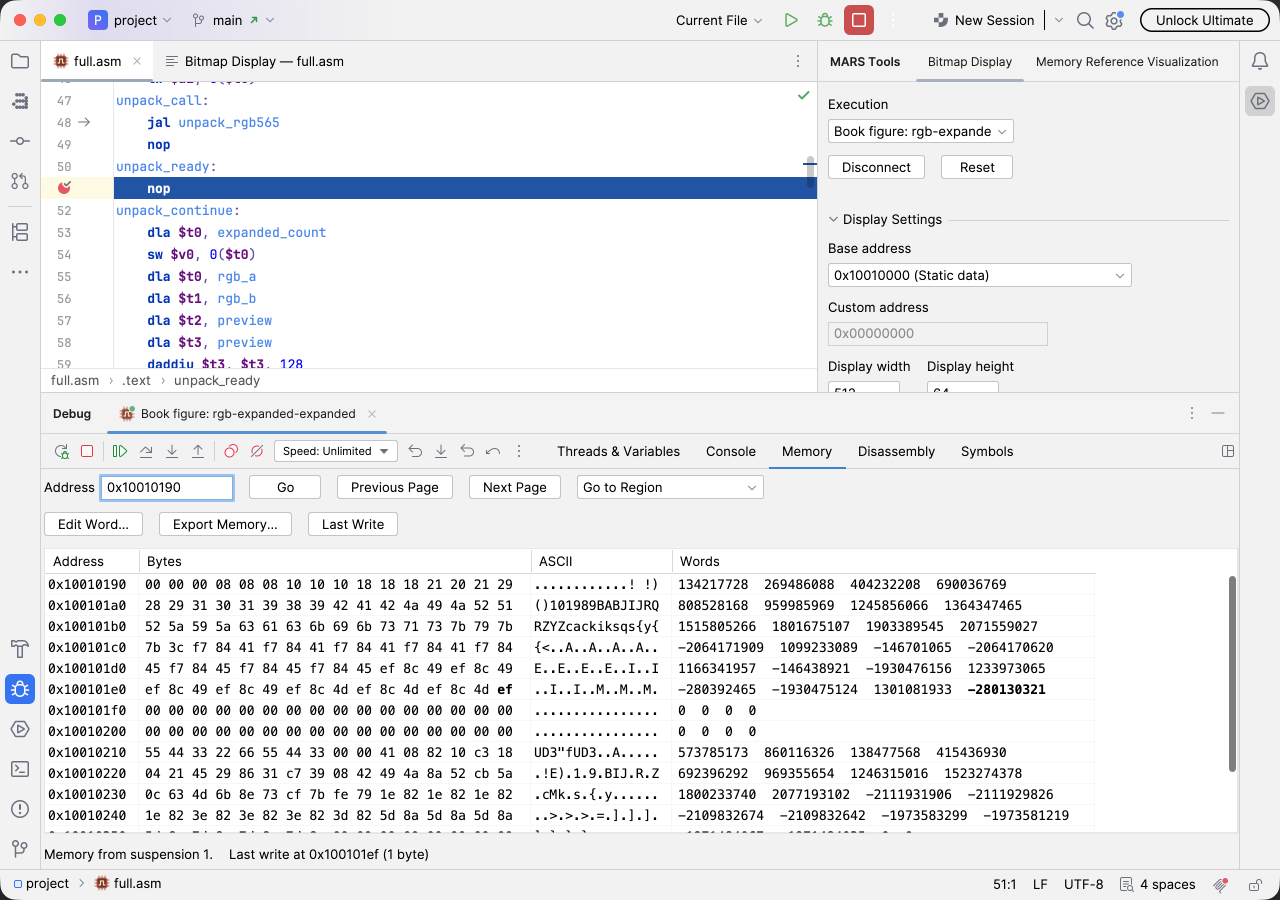
\includegraphics[artifact]{packages/019-rgb-formats/captures/f02/expanded.png}}
  \sbox6{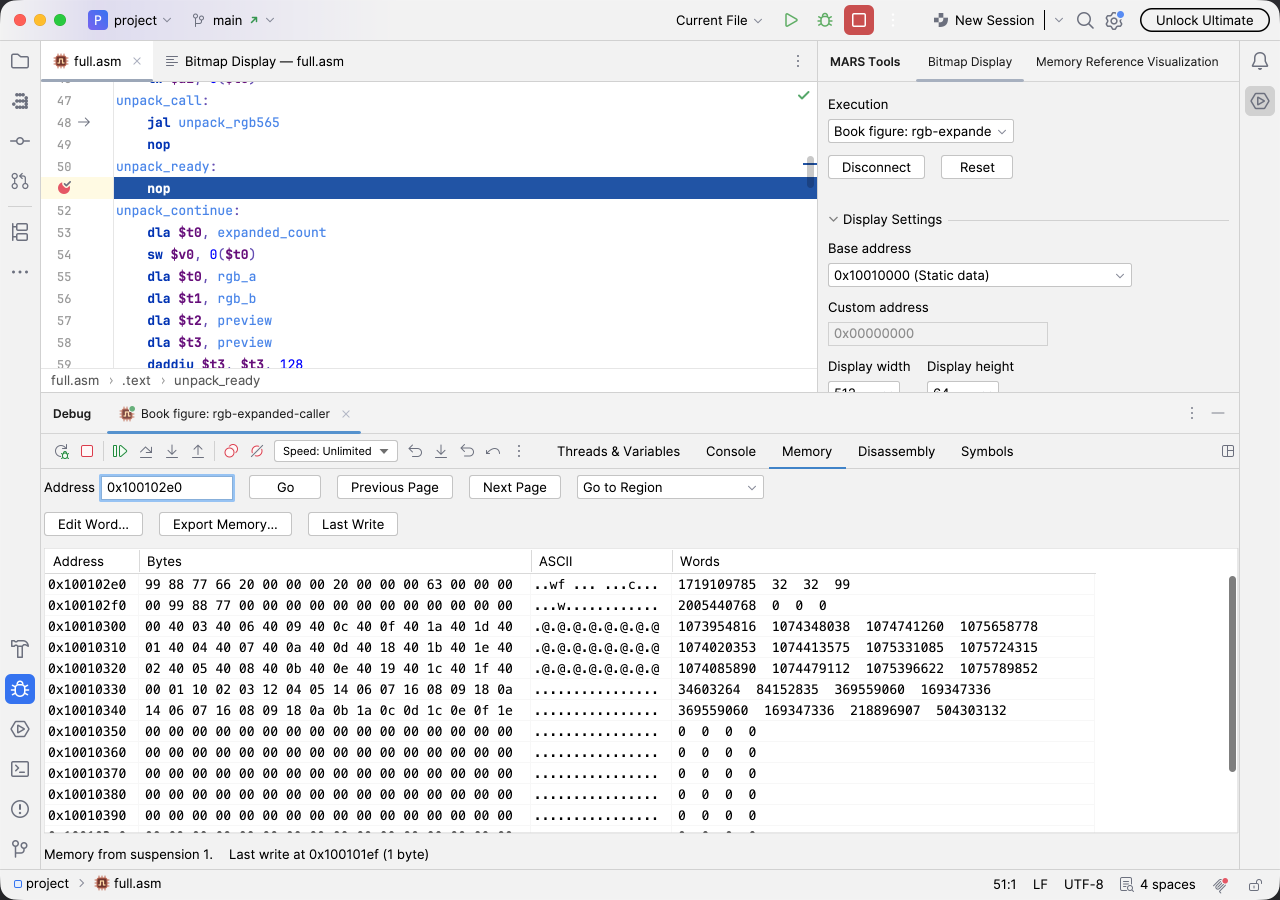
\includegraphics[artifact]{packages/019-rgb-formats/captures/f02/caller.png}}
  \edef\MARSrgbexpandedsourceLeft{\the\dimexpr0.036718750\wd0\relax}
  \edef\MARSrgbexpandedsourceBottom{\the\dimexpr0.774444444\ht0\relax}
  \edef\MARSrgbexpandedsourceRight{\the\dimexpr0.713281250\wd0\relax}
  \edef\MARSrgbexpandedsourceTop{\the\dimexpr0.170000000\ht0\relax}
  \edef\MARSrgbexpandedregistersLeft{\the\dimexpr0.246093750\wd0\relax}
  \edef\MARSrgbexpandedregistersBottom{\the\dimexpr0.334444444\ht0\relax}
  \edef\MARSrgbexpandedregistersRight{\the\dimexpr0.553906250\wd0\relax}
  \edef\MARSrgbexpandedregistersTop{\the\dimexpr0.640000000\ht0\relax}
  \edef\MARSrgbexpandedpackedLeft{\the\dimexpr0.034375000\wd2\relax}
  \edef\MARSrgbexpandedpackedBottom{\the\dimexpr0.311111111\ht2\relax}
  \edef\MARSrgbexpandedpackedRight{\the\dimexpr0.584375000\wd2\relax}
  \edef\MARSrgbexpandedpackedTop{\the\dimexpr0.608888889\ht2\relax}
  \edef\MARSrgbexpandedexpandedLeft{\the\dimexpr0.034375000\wd4\relax}
  \edef\MARSrgbexpandedexpandedBottom{\the\dimexpr0.311111111\ht4\relax}
  \edef\MARSrgbexpandedexpandedRight{\the\dimexpr0.584375000\wd4\relax}
  \edef\MARSrgbexpandedexpandedTop{\the\dimexpr0.608888889\ht4\relax}
  \edef\MARSrgbexpandedcallerLeft{\the\dimexpr0.034375000\wd6\relax}
  \edef\MARSrgbexpandedcallerBottom{\the\dimexpr0.334444444\ht6\relax}
  \edef\MARSrgbexpandedcallerRight{\the\dimexpr0.584375000\wd6\relax}
  \edef\MARSrgbexpandedcallerTop{\the\dimexpr0.608888889\ht6\relax}
  \begin{tikzpicture}[alt={Five annotated panels at unpack_ready show returned count 32, packed RGB565 bytes, expanded RGB triples and caller fields 32, 32, 99. The first expanded pixel is black, the second is eight, eight, eight. All 96 expanded bytes are complete, while the preview remains zero and the original RGB source is unchanged.}]
    \node[anchor=north west,inner sep=0,font=\small\bfseries] (source-title) at (6mm,0) {Next instruction at this boundary};
    \node[anchor=north west,inner sep=0] (source) at ([yshift=-1mm]source-title.south west) {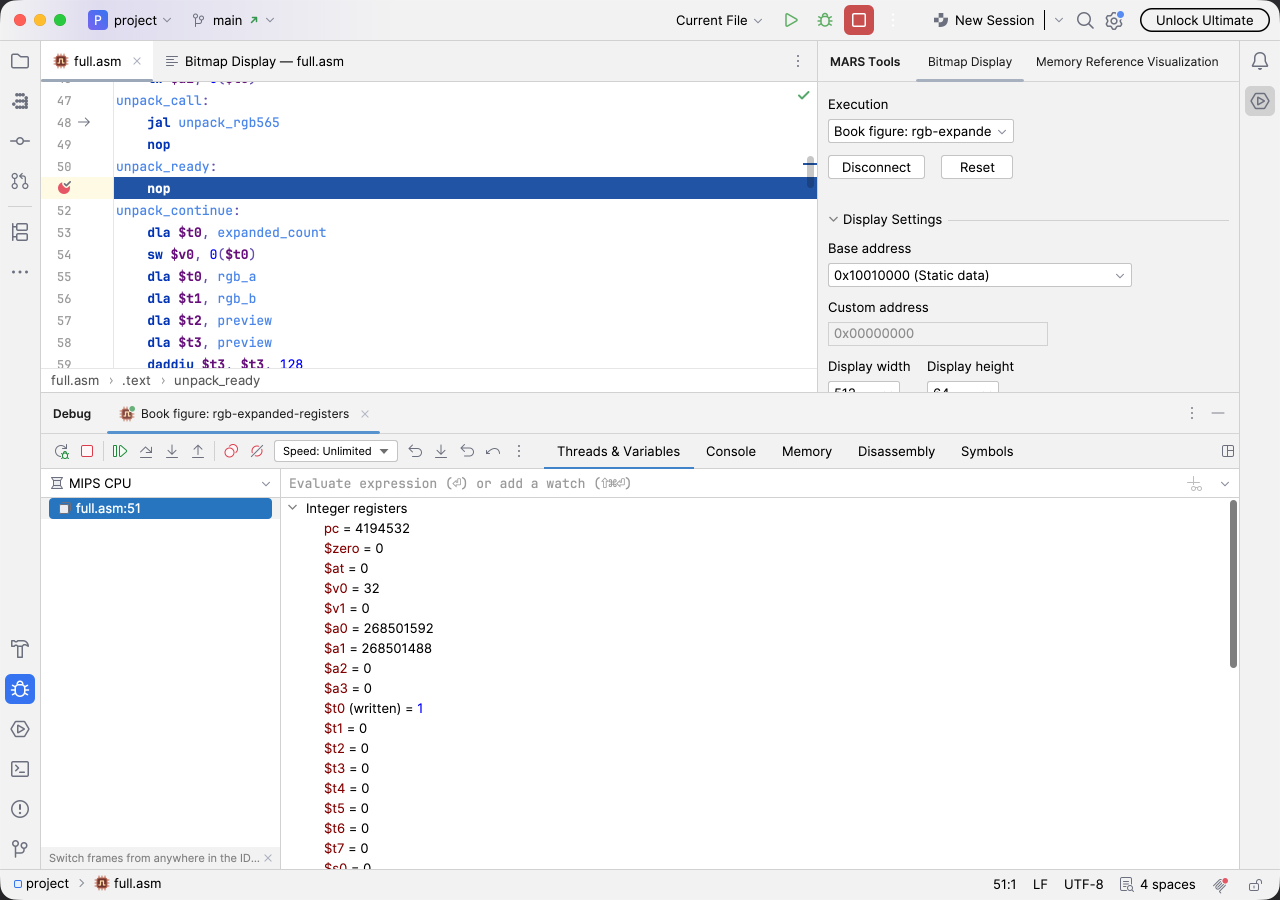
\includegraphics[width=0.54\linewidth,artifact,trim={\MARSrgbexpandedsourceLeft{} \MARSrgbexpandedsourceBottom{} \MARSrgbexpandedsourceRight{} \MARSrgbexpandedsourceTop{}},clip]{packages/019-rgb-formats/captures/f02/registers.png}};
    \begin{scope}[shift={(source.south west)},x={($(source.south east)-(source.south west)$)},y={($(source.north west)-(source.south west)$)}]
      \draw[black,line width=0.7pt] (0.215625000,0.080000000) rectangle (0.384375000,0.520000000);
      \node[draw=black,fill=white,circle,inner sep=1.5pt,font=\footnotesize] at ($(0.215625000,0.520000000)+(-3mm,0)$) {1};
    \end{scope}
    \node[anchor=north west,inner sep=0,font=\small\bfseries] (registers-title) at (0.58\linewidth,0 |- source-title.north) {Returned pixel count};
    \node[anchor=north west,inner sep=0] (registers) at ([yshift=-1mm]registers-title.south west) {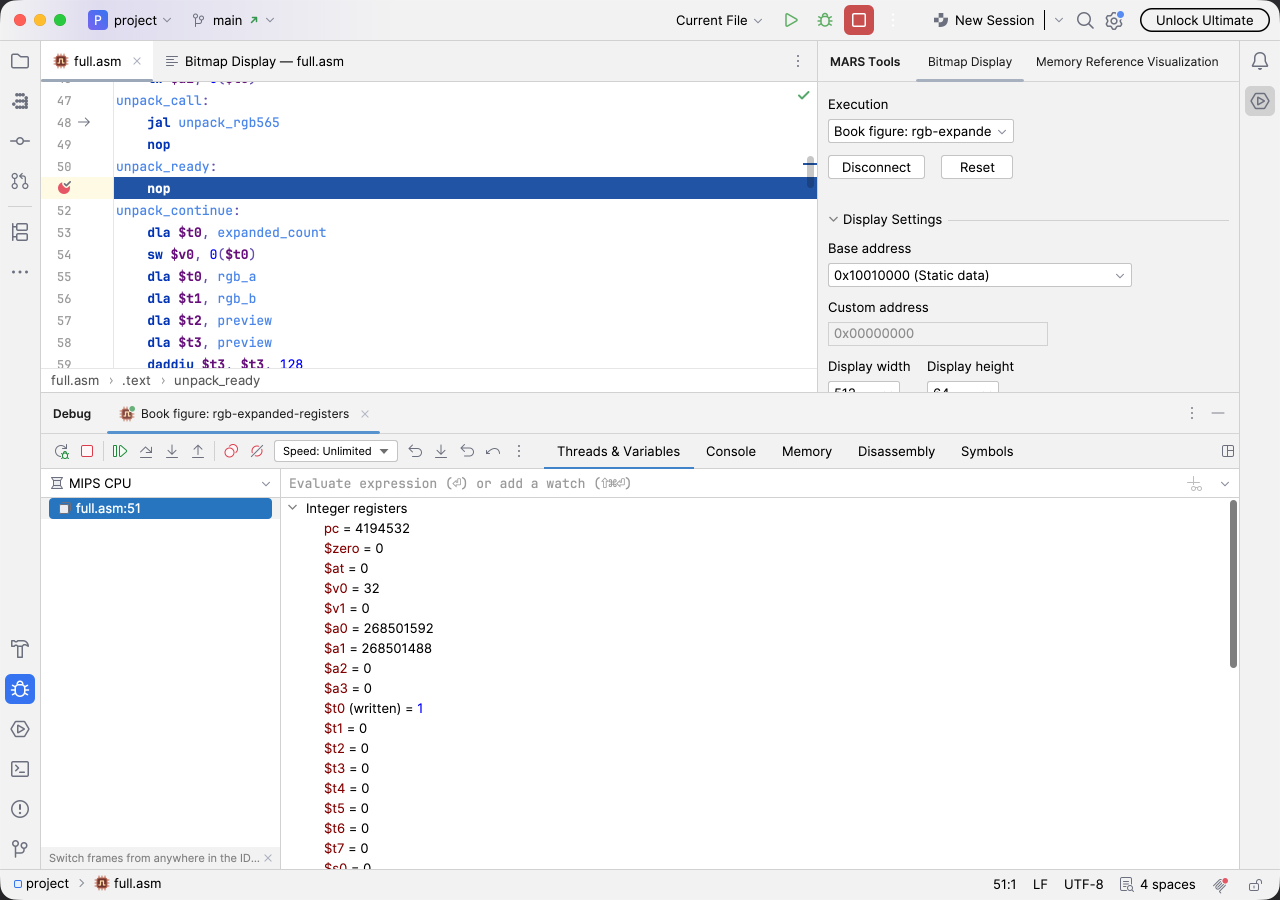
\includegraphics[width=0.42\linewidth,artifact,trim={\MARSrgbexpandedregistersLeft{} \MARSrgbexpandedregistersBottom{} \MARSrgbexpandedregistersRight{} \MARSrgbexpandedregistersTop{}},clip]{packages/019-rgb-formats/captures/f02/registers.png}};
    \begin{scope}[shift={(registers.south west)},x={($(registers.south east)-(registers.south west)$)},y={($(registers.north west)-(registers.south west)$)}]
      \draw[black,line width=0.7pt] (0.023437500,0.043478261) rectangle (0.257812500,0.913043478);
      \node[draw=black,fill=white,circle,inner sep=1.5pt,font=\footnotesize] at ($(0.023437500,0.913043478)+(-3mm,0)$) {2};
    \end{scope}
    \node[anchor=north west,inner sep=0,font=\small\bfseries] (packed-title) at ([yshift=-1mm]source.south west) {Low-byte-first RGB565};
    \node[anchor=north west,inner sep=0] (packed) at ([yshift=-1mm]packed-title.south west) {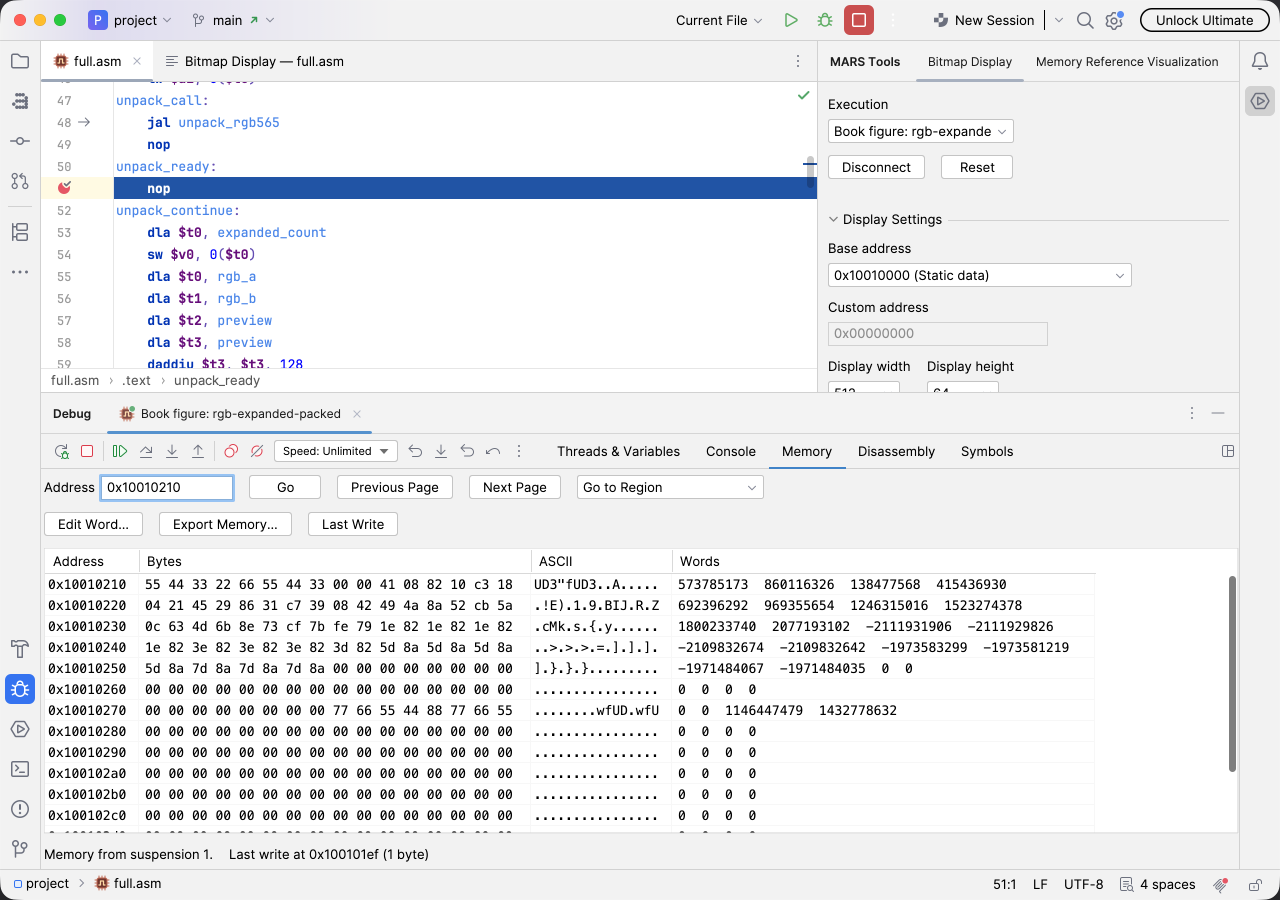
\includegraphics[width=0.84\linewidth,artifact,trim={\MARSrgbexpandedpackedLeft{} \MARSrgbexpandedpackedBottom{} \MARSrgbexpandedpackedRight{} \MARSrgbexpandedpackedTop{}},clip]{packages/019-rgb-formats/captures/f02/packed.png}};
    \begin{scope}[shift={(packed.south west)},x={($(packed.south east)-(packed.south west)$)},y={($(packed.north west)-(packed.south west)$)}]
      \draw[black,line width=0.7pt] (0.194672131,0.055555556) rectangle (0.997950820,0.638888889);
      \node[draw=black,fill=white,circle,inner sep=1.5pt,font=\footnotesize] at ($(0,0.638888889)+(-3mm,0)$) {3};
    \end{scope}
    \node[anchor=north west,inner sep=0,font=\small\bfseries] (expanded-title) at ([yshift=-1mm]packed.south west) {Expanded RGB component bytes};
    \node[anchor=north west,inner sep=0] (expanded) at ([yshift=-1mm]expanded-title.south west) {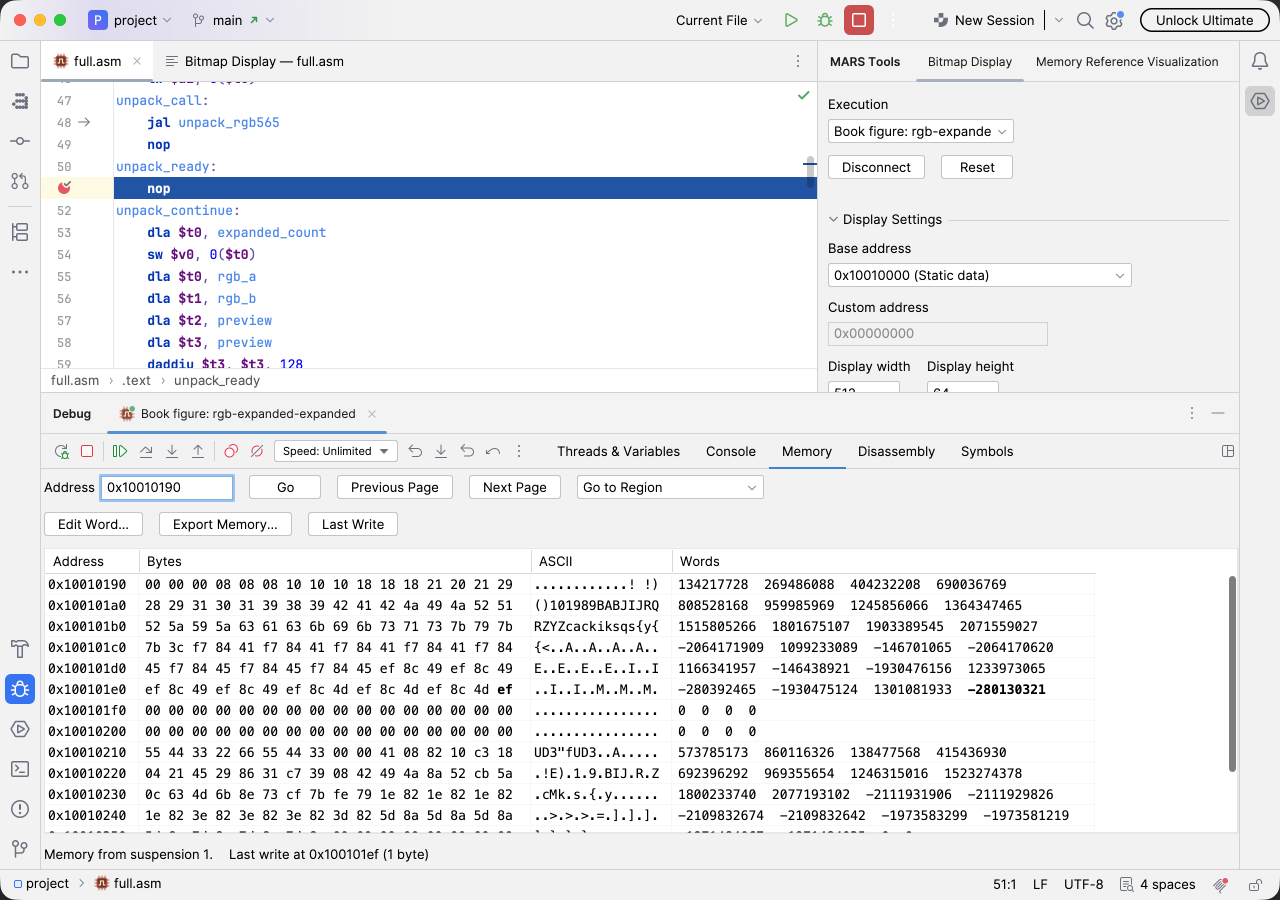
\includegraphics[width=0.84\linewidth,artifact,trim={\MARSrgbexpandedexpandedLeft{} \MARSrgbexpandedexpandedBottom{} \MARSrgbexpandedexpandedRight{} \MARSrgbexpandedexpandedTop{}},clip]{packages/019-rgb-formats/captures/f02/expanded.png}};
    \begin{scope}[shift={(expanded.south west)},x={($(expanded.south east)-(expanded.south west)$)},y={($(expanded.north west)-(expanded.south west)$)}]
      \draw[black,line width=0.7pt] (0.194672131,0.055555556) rectangle (0.997950820,0.638888889);
      \node[draw=black,fill=white,circle,inner sep=1.5pt,font=\footnotesize] at ($(0,0.638888889)+(-3mm,0)$) {4};
    \end{scope}
    \node[anchor=north west,inner sep=0,font=\small\bfseries] (caller-title) at ([yshift=-1mm]expanded.south west) {Count and caller result words};
    \node[anchor=north west,inner sep=0] (caller) at ([yshift=-1mm]caller-title.south west) {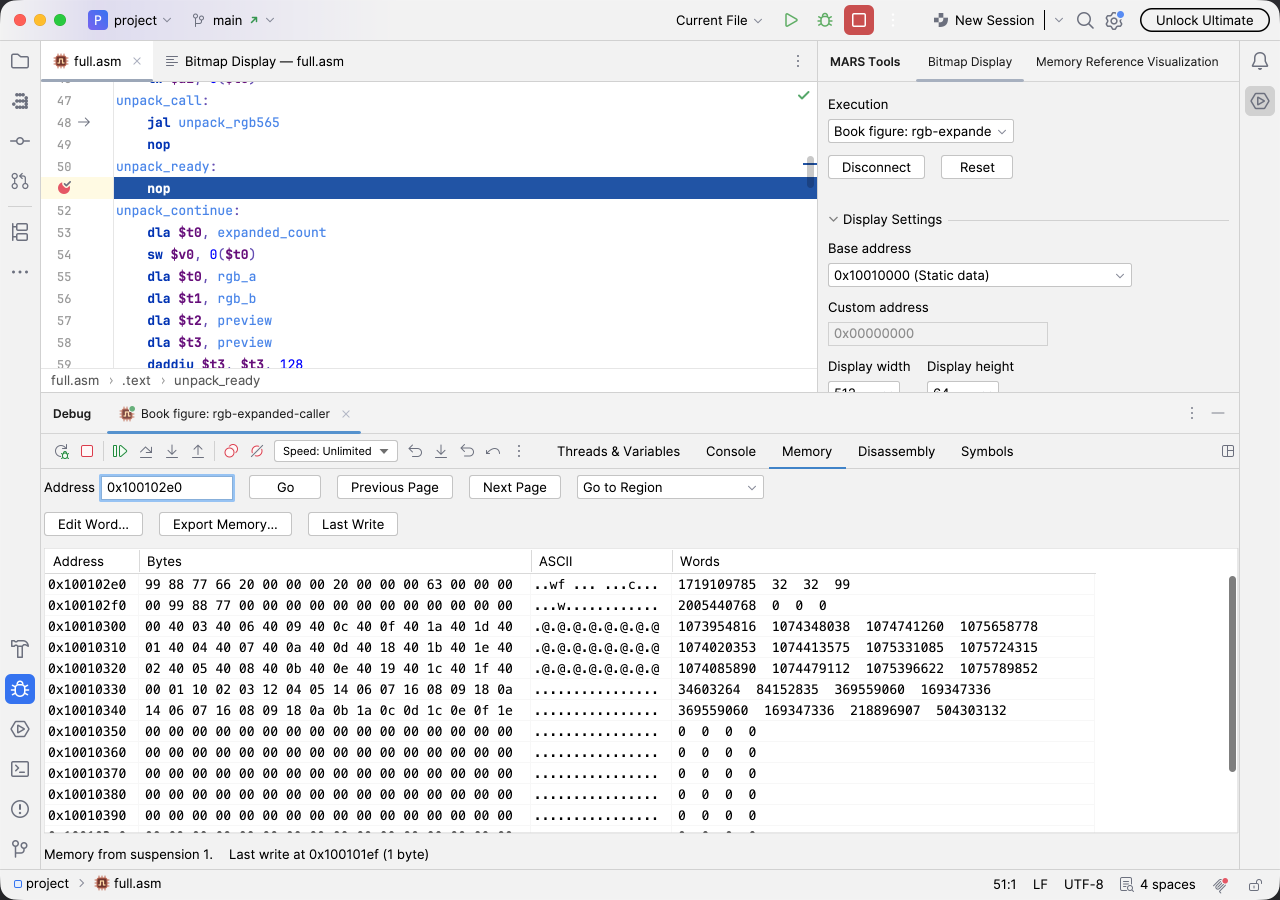
\includegraphics[width=0.84\linewidth,artifact,trim={\MARSrgbexpandedcallerLeft{} \MARSrgbexpandedcallerBottom{} \MARSrgbexpandedcallerRight{} \MARSrgbexpandedcallerTop{}},clip]{packages/019-rgb-formats/captures/f02/caller.png}};
    \begin{scope}[shift={(caller.south west)},x={($(caller.south east)-(caller.south west)$)},y={($(caller.north west)-(caller.south west)$)}]
      \draw[black,line width=0.7pt] (0.194672131,0.078431373) rectangle (0.997950820,0.490196078);
      \node[draw=black,fill=white,circle,inner sep=1.5pt,font=\footnotesize] at ($(0,0.490196078)+(-3mm,0)$) {5};
    \end{scope}
  \end{tikzpicture}
  \par\smallskip
  \begin{minipage}{\linewidth}
    \small
    \begin{enumerate}
      \setlength{\itemsep}{2pt}
            \setlength{\parsep}{0pt}
      \item The blue \texttt{nop} at \texttt{unpack\_ready} follows expansion. The caller has already stored the packing result, but has not stored the expansion result or built any preview word.
      \item \texttt{\$v0 = 32} again counts pixels. Expansion reads 64 packed bytes and produces 96 RGB component bytes. The input and output sizes exchange roles; the return value does not.
      \item The unchanged packed slice begins at \texttt{0x10010218}. Its first values are zero and \texttt{0x0841}. Reading bytes \texttt{41 08} unsigned and combining low plus 256 times high recovers the latter value before field extraction.
      \item Expanded RGB starts at \texttt{0x10010190}. The first triples are $(0,0,0)$, $(8,8,8)$, $(16,16,16)$ and $(24,24,24)$. A zero triple can be completed output: byte values alone do not distinguish black from an unfinished buffer. Length and the return boundary establish completion.
      \item The caller row now contains count 32, packed result 32 and expanded result 99 after its guard. Original RGB and packed input are preserved. The preview remains zero because its separate caller loop is still ahead.
    \end{enumerate}
  \end{minipage}
  \caption{Expansion repeats retained bits before the caller stores its second result.}
  \label{capture:019-rgb-formats-f02}
  \label{rgb-f02}
\end{figure}
\par
